\documentclass[11pt,a4paper]{article}

\usepackage[margin=1in]{geometry}
\usepackage{titlesec}
\usepackage{enumitem}
\usepackage{hyperref}
\usepackage{parskip}
\usepackage{graphicx}
\usepackage{float}
\usepackage{booktabs}
\usepackage{amsmath}

\hypersetup{colorlinks=true, linkcolor=blue, urlcolor=blue}

\titleformat{\section}{\large\bfseries}{\thesection}{0.5em}{}
\titleformat{\subsection}{\normalsize\bfseries}{\thesubsection}{0.5em}{}
\setlist{leftmargin=1.4em, topsep=2pt, itemsep=2pt}

\title{\vspace{-1.5cm}\textbf{PKCERT AI \& Software Development Internship \\ Task 11: Comparative Analysis of Classification Models}}
\author{Abdullah Amir}
\date{AI and Software Development \\ 16 July 2026}

\begin{document}

\maketitle
\vspace{-0.8cm}

This report covers the theory and the results. The full code, outputs and plots live in
the notebook \texttt{model\_comparison.ipynb}. The dataset is \textbf{UCI's Predict
Students' Dropout and Academic Success}: real administrative records for 4,424 students
at a Portuguese university, where the job is to predict whether a student will
\textbf{drop out}, remain \textbf{enrolled}, or \textbf{graduate}. Three models,
Logistic Regression, Random Forest and an SVM, are trained and tested on exactly the
same data and compared. The headline finding is one worth stating up front: the
\emph{simplest} of the three wins, and the metric you choose decides whether you can
see that at all.

% ----------------------------------------------------------------
\section*{Part A: Dataset Selection \& Preparation}

\textbf{The features.} Each of the 4,424 rows is one student described by 36 features,
which fall into four natural groups. There are \textbf{demographics} (age at enrolment,
gender, marital status, nationality, whether the student is displaced),
\textbf{family background} (the mother's and father's qualifications and occupations),
the \textbf{admission route} (application mode and order, the course applied for, the
previous qualification and its grade, the admission grade), and
\textbf{academic performance}. That last group is the important one: for each of the
first two semesters we know how many curricular units the student enrolled in, sat
evaluations for, and \textbf{passed}, along with their average grade. A few financial
signals sit alongside: scholarship holder, debtor, and whether tuition fees are up to
date.

\textbf{The target} is a genuine three-class variable: \texttt{Dropout} (1,421 students,
32.1 percent), \texttt{Enrolled} (794, 17.9 percent) and \texttt{Graduate} (2,209, 49.9
percent). The classes are imbalanced, and the middle one is awkward by construction:
``Enrolled'' does not describe an outcome at all, it describes a student whose outcome
has not happened yet. That single fact ends up driving every result in this report.

\textbf{Preprocessing.} There are no missing values, so the real work is deciding what
each column actually \emph{means}, and two decisions matter.

\begin{itemize}
    \item \textbf{Some ``numbers'' are not numbers.} Columns such as \texttt{Course},
    \texttt{Application mode} and \texttt{Mother's occupation} are stored as integer
    codes standing in for categories. Left alone, a linear model would read them as
    quantities and cheerfully conclude that ``Course 12 is greater than Course 3'',
    which is meaningless. These nine columns are \textbf{one-hot encoded}, which expands
    the 36 original columns into 236 model features.
    \item \textbf{Scaling.} Ages, grades and unit counts live on very different scales.
    Logistic Regression and especially the SVM are sensitive to that; the Random Forest
    is not, because a tree only ever asks whether a value sits above some threshold.
    Standardising is essential for two of the three models and harmless to the third.
\end{itemize}

Both steps live in a single \texttt{ColumnTransformer} wrapped into a
\texttt{Pipeline} with each model. This matters twice over. It makes the comparison
\emph{fair}, since every model sees identical inputs, and it makes it \emph{correct},
because the scaler and encoder are fit on the training fold only, so nothing leaks back
from the test set. We split 80/20 with stratification, leaving 3,539 students for
training and 885 for testing, with the class proportions preserved on both sides.

\begin{figure}[H]
    \centering
    
\includegraphics[width=0.9\textwidth]{figures/01_dataset_overview.png}
    \caption{Left: the three-way target, with \texttt{Enrolled} the clear minority at
    17.9 percent. Right: admission grade by outcome. The boxes overlap almost
    completely, so how a student \emph{started} says very little about how they finish.}
\end{figure}

\begin{figure}[H]
    \centering
    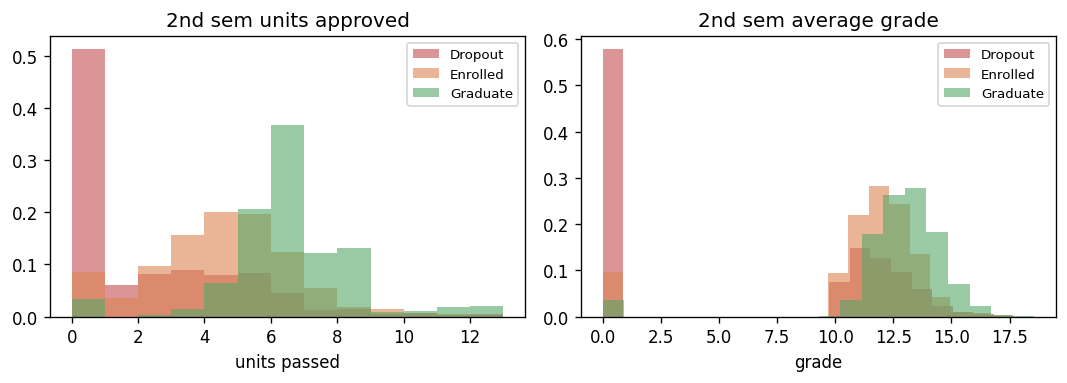
\includegraphics[width=0.9\textwidth]{figures/02_key_features.png}
    \caption{Where the signal actually lives. Dropouts pile up at zero units passed
    while graduates cluster at five or six. Note that \texttt{Enrolled} students sit
    \emph{between} the two and overlap both, which is why the middle class is so hard
    for every model.}
\end{figure}

% ----------------------------------------------------------------
\section*{Part B: Model Development}

All three models are built on the shared pipeline described above and trained on the
same 3,539 students.

\textbf{Logistic Regression} is a \textbf{linear} model. It takes a weighted sum of the
features and pushes it through a softmax to produce a probability for each of the three
classes, learning the weights by maximising the likelihood of the outcomes actually
observed. Its boundaries between classes are straight lines (strictly, hyperplanes),
which sounds like a crippling restriction and turns out not to be.

\textbf{Random Forest} is an \textbf{ensemble} of 300 decision trees. Each tree is grown
on a bootstrap sample of the rows and may only consider a random subset of the features
at each split, so the trees make different mistakes and averaging their votes cancels
out much of the noise a single tree would suffer. It picks up non-linear patterns and
feature interactions without being asked, and needs no scaling.

\textbf{SVM} with an \textbf{RBF kernel} looks for the boundary that separates the
classes with the widest possible \textbf{margin}, where only the points on the edge of
that gap, the \textbf{support vectors}, determine where it lands. The kernel trick lets
that boundary bend into non-linear shapes without ever computing the higher dimensional
coordinates explicitly. It is the most scaling-sensitive of the three, which the shared
pipeline already takes care of.

\textbf{On the choice of metric.} We report \textbf{macro} averages for precision,
recall and F1. Macro treats all three classes as equally important no matter how many
students are in each, so a model cannot look good simply by nailing the large
\texttt{Graduate} class and quietly writing off the small \texttt{Enrolled} one. As Part
C shows, that choice is the difference between seeing what happened and missing it
entirely.

% ----------------------------------------------------------------
\section*{Part C: Model Evaluation \& Comparison}

\begin{table}[H]
\centering
\begin{tabular}{lrrrrrr}
\toprule
\textbf{Model} & \textbf{Accuracy} & \textbf{Precision} & \textbf{Recall} & \textbf{F1} & \textbf{F1 (wtd)} & \textbf{CV F1 (std)} \\
 & & \textbf{(macro)} & \textbf{(macro)} & \textbf{(macro)} & & \\
\midrule
Logistic Regression & 0.7672 & 0.7122 & 0.6847 & \textbf{0.6930} & 0.7563 & \textbf{0.701} (0.012) \\
Random Forest       & 0.7672 & 0.7188 & 0.6572 & 0.6625 & 0.7410 & 0.672 (0.006) \\
SVM (RBF kernel)    & 0.7605 & 0.7086 & 0.6732 & 0.6839 & 0.7484 & 0.690 (0.006) \\
\bottomrule
\end{tabular}
\caption{All three models on identical data and the same 80/20 split. The last column
is 5-fold cross-validated macro F1 over the full dataset.}
\end{table}

\begin{figure}[H]
    \centering
    
\includegraphics[width=0.95\textwidth]{figures/03_confusion_matrices.png}
    \caption{Confusion matrices. Rows are the true outcome, columns the prediction. The
    middle row, real \texttt{Enrolled} students, is where the three models genuinely
    part company.}
\end{figure}

\begin{figure}[H]
    \centering
    
\includegraphics[width=0.66\textwidth]{figures/04_model_comparison.png}
    \caption{The four headline metrics. Accuracy is effectively a three-way tie; macro
    F1 is not.}
\end{figure}

\textbf{Accuracy hides the entire story.} Logistic Regression and Random Forest tie at
\emph{exactly} 0.7672. Had we stopped at accuracy, as the brief's first metric, we would
have called it a dead heat and moved on. Macro F1 disagrees sharply: 0.6930 for Logistic
Regression against 0.6625 for the forest. Something is going on that accuracy cannot
see, and the per-class recall says what.

\begin{table}[H]
\centering
\begin{tabular}{lrrr}
\toprule
\textbf{Recall per class} & \textbf{Logistic Regression} & \textbf{Random Forest} & \textbf{SVM} \\
\midrule
Dropout  & 0.750 & \textbf{0.768} & 0.715 \\
Enrolled & \textbf{0.390} & 0.252 & 0.377 \\
Graduate & 0.914 & \textbf{0.952} & 0.928 \\
\bottomrule
\end{tabular}
\caption{The \texttt{Enrolled} row is the whole difference between the models.}
\end{table}

\begin{figure}[H]
    \centering
    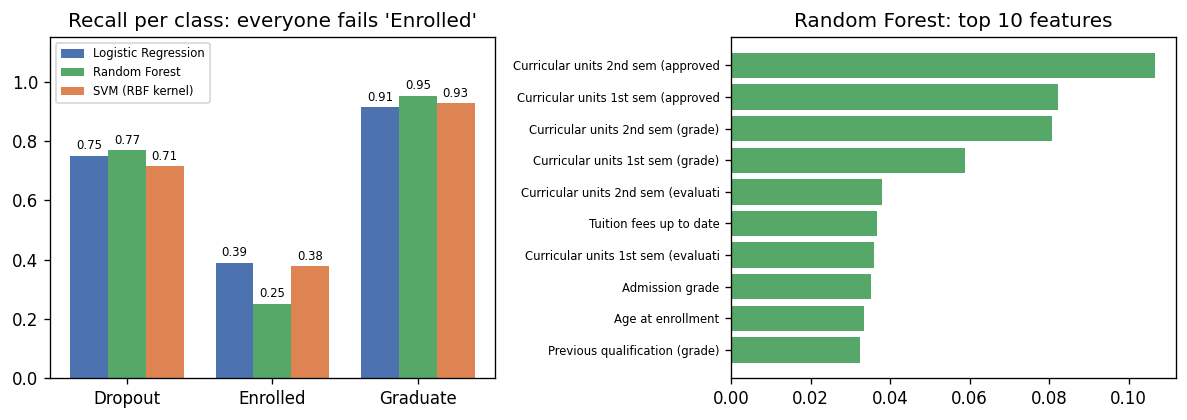
\includegraphics[width=0.95\textwidth]{figures/05_perclass_and_importance.png}
    \caption{Left: recall per class. Every model struggles with \texttt{Enrolled}, but
    the forest struggles most. Right: the forest's top ten features, dominated by
    semester units passed and grades.}
\end{figure}

\textbf{The \texttt{Enrolled} class is where it is decided.} The Random Forest recovers
only \textbf{25.2 percent} of still-enrolled students, against Logistic Regression's
\textbf{39.0 percent}. The forest has effectively given up on the hard minority class
and banked the easy wins instead, and it is the best of the three at
\texttt{Graduate} (95.2 percent recall) and at \texttt{Dropout} (76.8 percent) as a
result. Because \texttt{Graduate} is half the dataset, that trade costs it almost
nothing in accuracy while gutting its macro F1. This is precisely the failure mode macro
averaging exists to expose, and it is why the choice of metric in Part B mattered.

\textbf{Cross-validation confirms this is not a fluke of one split.} Logistic Regression
leads on 5-fold macro F1 with 0.701, ahead of the SVM's 0.690 and the forest's 0.672.
The forest's deficit of roughly 0.03 is about five times its own fold-to-fold standard
deviation of 0.006, so this is a real gap rather than noise. It is worth being careful
here: the gap between Logistic Regression and the SVM is a slimmer 0.011 against a
spread of 0.012, so those two are much closer to tied than the ordering suggests.

\textbf{Why the simplest model wins.} The forest's own feature importances give the
answer. The top features are overwhelmingly second and first semester units approved and
the associated grades, and that relationship is close to \textbf{monotonic}: pass more
units, more likely to graduate. A linear model represents a monotonic relationship
perfectly. The forest's and the SVM's extra flexibility therefore has almost no genuine
non-linear structure left to discover, so that capacity goes into fitting noise instead,
which is exactly what overfitting is.

\subsection*{Strengths and weaknesses}

\textbf{Logistic Regression.} \emph{Strengths:} the best macro F1 and the best
cross-validated score here; fast to train; produces well calibrated probabilities; and
its coefficients are directly interpretable, so you can say precisely why a given
student was flagged. \emph{Weaknesses:} it can only draw linear boundaries, so on
genuinely non-linear data it would lose badly; it needs feature scaling; and it is
sensitive to strongly correlated features, of which this dataset has several (first and
second semester results move together).

\textbf{Random Forest.} \emph{Strengths:} the best \texttt{Dropout} recall and the best
\texttt{Graduate} recall; needs no scaling; captures interactions automatically; and it
hands you feature importances for free, which is how we diagnosed the dataset in the
first place. \emph{Weaknesses:} the worst macro F1 of the three here; it abandoned the
minority class; 300 averaged trees are not interpretable in any practical sense; and it
is the slowest to train.

\textbf{SVM (RBF).} \emph{Strengths:} a solid middle finisher, second on both macro F1
and cross-validation; strong in high dimensional spaces, which suits our 236 encoded
features; and the maximum-margin objective generalises well. \emph{Weaknesses:} it gives
no probabilities without extra expense; it is the most scaling-dependent of the three;
\texttt{C} and \texttt{gamma} really need tuning for it to shine, and we left them at
defaults; and it scales poorly to much larger datasets.

% ----------------------------------------------------------------
\section*{Part D: Recommendation \& Conclusion}

\textbf{Recommendation: Logistic Regression.} The justification comes straight from the
evaluation results above.

\begin{enumerate}
    \item \textbf{It has the best macro F1} on the held-out test set, 0.6930 against the
    SVM's 0.6839 and the forest's 0.6625. Macro F1 is the right yardstick here precisely
    because it refuses to let a model ignore the small \texttt{Enrolled} class.
    \item \textbf{Cross-validation backs it up.} Its 5-fold macro F1 of 0.701 leads both
    rivals, so the win survives resampling instead of resting on one lucky split.
    \item \textbf{It handles the hard class best}, recovering 39.0 percent of
    \texttt{Enrolled} students against the forest's 25.2 percent.
    \item \textbf{It is by far the most interpretable.} That is not a tiebreaker here,
    it is a requirement. A university acting on these predictions has to be able to tell
    a student, or an auditor, why they were flagged, and a coefficient does that where
    300 averaged trees cannot.
\end{enumerate}

\textbf{The honest caveats.} On accuracy alone this is a three-way tie (0.767, 0.767,
0.761) and none of the above would matter, which is itself the lesson rather than an
inconvenience. The Logistic Regression and SVM gap is inside one standard deviation of
the cross-validation spread, so calling Logistic Regression the winner over the SVM is a
weaker claim than calling it the winner over the forest. And if the goal were narrowly
``catch as many likely dropouts as possible so we can intervene early'', then the
\textbf{Random Forest} would be the better choice, since its \texttt{Dropout} recall of
76.8 percent beats Logistic Regression's 75.0 percent. The right model genuinely depends
on which mistake you are trying not to make.

\textbf{Conclusion.} The most useful finding from this comparison is that the
\emph{simplest model won}. The dominant signal in this data, pass your units and you
graduate, is close to linear, so the extra flexibility of the forest and the SVM bought
nothing at all, and in the forest's case it actively hurt. Model complexity is not a
ladder you climb until the score improves; it is a choice that should match the shape of
the data, and here the data is simple. All three models also agree on the deeper problem
in this dataset, which no algorithm can fix: \texttt{Enrolled} is genuinely ambiguous,
because those students have not finished yet, and their features look like a blend of
the two real outcomes. No amount of model selection or tuning will resolve a label that
the future has not decided. The honest fix would be better data, following those
students until they graduate or leave, rather than a better classifier.

\vspace{0.4cm}
The notebook and README are on GitHub:
\url{https://github.com/AbdullahAmir06/ai-internship-abdullahamir}.

\end{document}
